\section{Improved Parallel Composition}\label{sec_intro}



\subsection{Abstract}
Parallel composition of labelled Petri nets is a fundamental operation in modular design. It is often used to combine models of subsystems into a model of the whole system.
Unfortunately, the standard definition of parallel composition almost always yields a `messy' Petri net, with many implicit places, causing performance deterioration in tools that are based on structural methods. In this paper we propose an optimised algorithm for computing the parallel composition. It often produces nets with fewer implicit places, which are thus better suited for subsequent application of structural methods.

\subsection{Introduction}

Parallel composition (\aka synchronous product) of labelled
Petri nets is a fundamental operation in modular design. It is
often used to combine models of subsystems into a model of the
whole system. In particular, there is a nice correspondence
between parallel composition of Signal Transition Graphs
(STGs), a class of labelled Petri nets used for modelling
asynchronous circuits, and connecting circuits by wires. Hence
performing this operation efficiently is important in practice.

Unfortunately, the standard definition of parallel composition almost always yields a `messy' Petri net, with many implicit places (even if the component Petri nets did not have them). Some of these places are easy to remove (\eg duplicate places, which have the same pre- and postsets), but in general for removing others one needs full-blown model checking, which is infeasible if the resulting composition is large.
Although implicit places do not have noticeable effect on tools based on state space exploration, such as \petrify~\cite{ckkly97}, the performance of tools that are based on structural methods, such as \desij~\cite{Sch07}, often deteriorates.

Consider an example shown in Fig.~\ref{fi-motivating-example1},
which shows the STG specifications of two components (a,b) and
the specification of the environment (c). (The used short-hand
drawing notation for STGs is explained in
Sect.~\ref{sec_pn_basic}.) The model of the behaviour of the
entire system can be obtained by constructing the parallel
composition of these three STGs, which is shown in part (d) of
this figure. One can see that it contains a few implicit places
(which are not duplicate places); intuitively, they appear due
to repeated causality specifications for every signal: the one
coming from the component where this signal is an output, and
others --- from the components where it is an input. Removing
these places yields a much `cleaner' STG, coinciding with that
shown in Fig.~\ref{fi-motivating-example2}(d).

\begin{figure}[!tb]
    \centering
    \begin{minipage}[b]{0.4\columnwidth}
    \centering
        $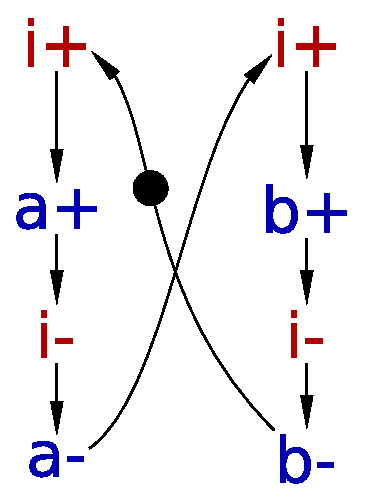
\includegraphics[scale=0.3]{EXPERIMENTS/stg/toggle}
        \atop
        \mbox{\rule[1.3em]{0em}{0em}(a) Toggle}$
        \\[0.5em]
        $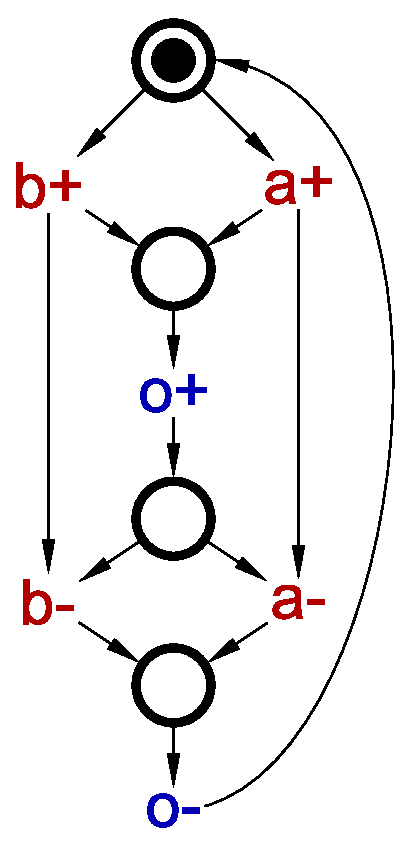
\includegraphics[scale=0.3]{EXPERIMENTS/stg/mix}
        \atop
        \mbox{\rule[1.3em]{0em}{0em}(b) Call}$
        \\[0.5em]
        $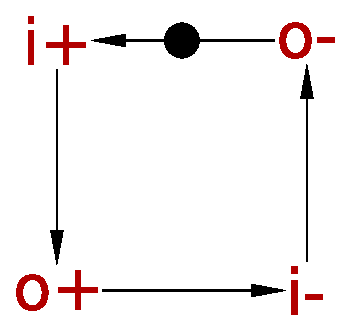
\includegraphics[scale=0.3]{EXPERIMENTS/stg/env}
        \atop
        \mbox{\rule[1.3em]{0em}{0em}(c) Environment}$
    \end{minipage}
    $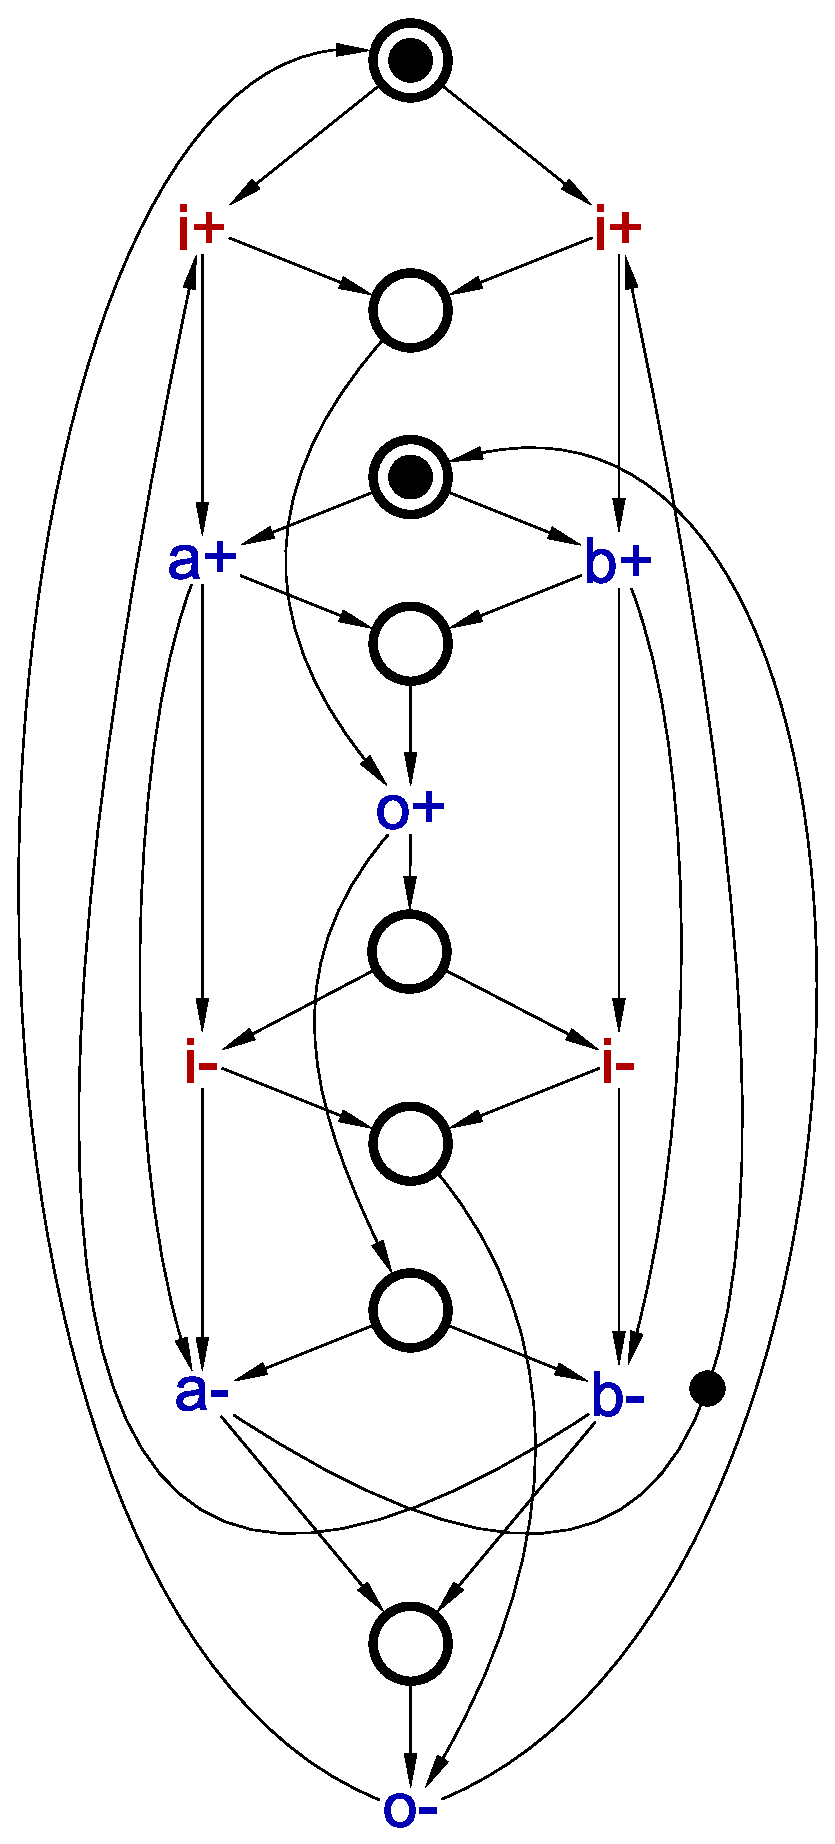
\includegraphics[scale=0.3]{EXPERIMENTS/stg/simple_standard}
    \atop
    \mbox{\rule[1.3em]{0em}{0em}(d) Composition}$
    \caption{\label{fi-motivating-example1}
        Example of standard STG composition.
    }
\end{figure}

\begin{figure}[!tb]
    \centering
    \begin{minipage}[b]{0.4\columnwidth}
        \centering
        $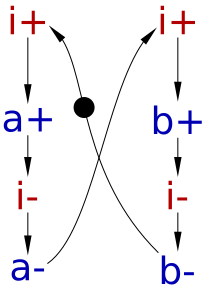
\includegraphics[scale=0.3]{EXPERIMENTS/stg/toggle_opt}
        \atop
        \mbox{\rule[1.3em]{0em}{0em}(a) Toggle}$
        \\[0.5em]
        $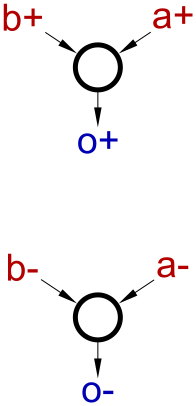
\includegraphics[scale=0.3]{EXPERIMENTS/stg/mix_opt}
        \atop
        \mbox{\rule[1.3em]{0em}{0em}(b) Call}$
        \\[0.5em]
        $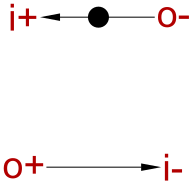
\includegraphics[scale=0.3]{EXPERIMENTS/stg/env_opt}
        \atop
        \mbox{\rule[1.3em]{0em}{0em}(c) Environment}$
    \end{minipage}
    $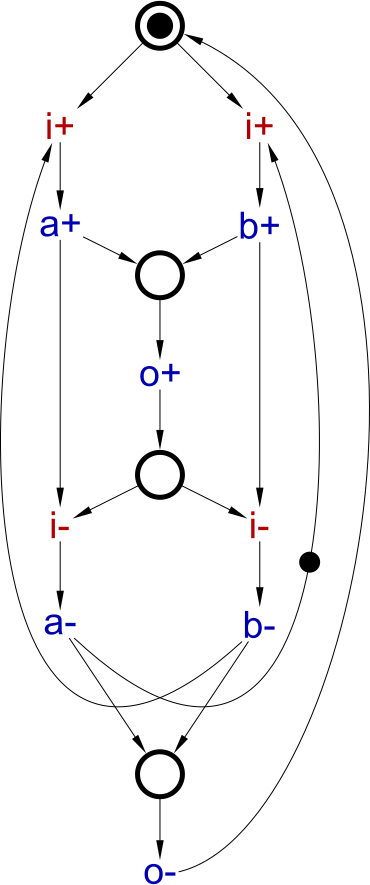
\includegraphics[scale=0.3]{EXPERIMENTS/stg/simple_improved}
    \atop
    \mbox{\rule[1.3em]{0em}{0em}(d) Composition}$
    \caption{\label{fi-motivating-example2}
        Example of improved STG composition: the components are obtained from the corresponding ones in Fig.~\ref{fi-motivating-example1} by removing some places, and then the standard parallel composition is applied to these modified components.
    }
\end{figure}


One operation where implicit places matter is \emph{transition contraction,}~\cite{vowo02lncs} which is a crucial part of the re-syn\-the\-sis approach~\cite{CN-02,KVL-96,PC-96}. The idea is to hide the internal communication between the components (by labelling the corresponding transitions as `dummy' --- they correspond to signals $a$ and $b$ in our example), contract as many of these dummy transitions as possible (whereby reducing the size of the STG), and re-synthesise the obtained STG as a circuit (which is often smaller than the original circuit due to removal of some signals). Transition contraction has to be performed on very large STGs (corresponding to the whole control path of the circuit), and so, for efficiency, it has to be a structural operation. Unfortunately, such structural contractions are not always possible (see Sect.~\ref{sec_pn_basic}), and implicit places in the preset and/or postset of a transition can prevent contracting it, even if a contraction is possible after removing these implicit places. In our example, \desij cannot contract any of the dummy transitions in the STG in Fig.~\ref{fi-motivating-example1}(d), even though it performs some structural tests for place redundancy; however, it is able to contract all the dummy transitions if the implicit places are removed, \ie when applied to the STG in Fig.~\ref{fi-motivating-example2}(d).

The main contribution of this paper is a new me\-thod for computing the parallel composition of labelled Petri nets, that generates fewer implicit places. It uses the \emph{freeness from computation interference (FCI)} assumption, stating that the situation when one component wants to produce an output, but is prevented from doing so by another component which is not ready to receive it, is impossible. Violation of FCI means that the behaviour of the composition does not correspond to that of the physical system. For example, an output of a circuit component cannot be physically disabled by another component that is not ready to receive this signal, and so producing this output will lead to malfunction; however, the composition will be oblivious to it, and behave as if such an output could not be produced.
Hence FCI is a basic correctness requirement --- if it is violated, there is no point in computing parallel composition, as its behaviour will not describe that of the physical system. In practice, FCI is often guaranteed by construction, \eg it is always guaranteed for the control path of a \balsa~\cite{EB-02} or \haste/\tangram~\cite{berkel91,haste-manual} specification of an asynchronous circuit. The idea of using the FCI condition is reminiscent of the method of input/output exposure in the synthesis by direct mapping described in~\cite{SBY-07}, and of the correct by construction composition of Petri nets for circuit components and the environment used in the \ditopn tool~\cite{JF-00}.

The main idea of the method we propose here is illustrated by the example in Fig.~\ref{fi-motivating-example2}. Before doing the parallel composition, one can remove some of the places in the components as shown in parts (a--c) of the figure and then compose the modified STGs. The precise conditions that allow to remove a particular place will be stated in Sect.~\ref{se-main}; at this point it is only important that they are structural and thus can be efficiently checked. This guarantees that the number of places in the resulting Petri net is smaller (as the number of places in the composition is the total number of places in all the components), and, under the FCI assumption, the resulting behaviour will be the same (in the sense of isomorphism of the reachability graphs). In particular, in our example, composing the modified components yields the STG in Fig.~\ref{fi-motivating-example2}(d), which in this case contains no implicit places. Observe that the modified components on their own can have rather bad behaviour and in particular can be non-implementable; however, it does not matter, as they are never used on their own, but only in composition with other components, and the resulting behaviour of the composition is guaranteed to correspond to that of the standard composition.

Re-synthesis of asynchronous circuits is the intended application of the proposed method. However, we envisage that it has a much wider applicability, as composition of labelled Petri nets is a fundamental operation, and the FCI assumption often holds in practice.
